\documentclass[10pt,a4paper]{article}
\usepackage[T1]{fontenc}
\usepackage[scaled]{helvet}
\usepackage{cite}
\usepackage{url}
\usepackage{graphicx}
\usepackage{listings}
\usepackage{float}
\usepackage{amsmath}
\usepackage{listings}
\usepackage{color}
 
\definecolor{dkgreen}{rgb}{0,0.6,0}
\definecolor{gray}{rgb}{0.5,0.5,0.5}
\definecolor{mauve}{rgb}{0.58,0,0.82}
\lstset{ %
  language=Octave,                % the language of the code
  basicstyle=\footnotesize,           % the size of the fonts that are used for the code
  numbers=left,                   % where to put the line-numbers
  numberstyle=\tiny\color{gray},  % the style that is used for the line-numbers
  stepnumber=1,                   % the step between two line-numbers. If it's 1, each line 
                                  % will be numbered
  numbersep=5pt,                  % how far the line-numbers are from the code
  backgroundcolor=\color{white},      % choose the background color. You must add \usepackage{color}
  showspaces=false,               % show spaces adding particular underscores
  showstringspaces=true,         % underline spaces within strings
  showtabs=false,                 % show tabs within strings adding particular underscores
  frame=none,                   % adds a frame around the code
  rulecolor=\color{black},        % if not set, the frame-color may be changed on line-breaks within not-black text (e.g. commens (green here))
  tabsize=2,                      % sets default tabsize to 2 spaces
  breaklines=true,                % sets automatic line breaking
  breakatwhitespace=false,        % sets if automatic breaks should only happen at whitespace
  keywordstyle=\color{blue},          % keyword style
  commentstyle=\color{dkgreen},       % comment style
  stringstyle=\color{mauve},         % string literal style
  escapeinside={\%*}{*)},            % if you want to add LaTeX within your code
  morekeywords={*,...}               % if you want to add more keywords to the set
}
\usepackage{amssymb}
\usepackage{fancyhdr}
\usepackage{lastpage}
\floatstyle{boxed} 
\restylefloat{figure}
\renewcommand*\familydefault{\sfdefault}
\title{Introduction to Algorithms}
\author{David Lynch - david.lynch@raglansoftware.com }
\begin{document}
\maketitle
\begin{abstract}
We shift or focus now from core operating systems to algorithms and data structures. Essentially, we pivot from looking at software and methods that facilitate the creation and running of programs to the actual construction of the programs themselves. We start with a gentle introduction to some primitive data-structures and put a formal framework around evaluating algorithms.
\end{abstract}
\section{Elementary Data Structures}
Dynamic sets are the fundamental structures to computer science. Strictly speaking, mathematical sets are unchanging, however in computer science it is useful to picture a set as a collection of values that actually mutates in some way over time. We make the distinction by calling these types of sets {\bf dynamic}. Algorithms may require several different types of operations to be performed on sets of data. We refer to sets that support these operations as {\bf dictionaries}. Operations that must be supported for particular dictionaries vary between data-structure, each of which will have its own set of operations that together make the structure unique. Dictionaries contain {\bf objects} of primitive data each of which is identified individually due to either their position in a set relative to the lower and upper bounds, that is by {\bf implicit key}, or by means of {\bf explicit key}. The explicit key is derived from some identiifying value or set of values that are associated with the object itself. An example implicit key is the position of an object reference in an array, whereas an explicit key may be a hash-code derived from the results of a hash function across the associated object. It is beneficial to think of dictionaries as sets of {\bf key-value pairs}. The data associated with an objeect that is unused by the set implementation itself is known as {\bf satellite data}. So, consider the example of an array of bank accounts. The key is the implicit position in the array, which maps to an object reference that resolves to the account number, name and balance. 
\newline\newline
If $S$ is a possibly ordered set and $k$ is a {\bf key} that points to some object $x$, anything that modifies the contents of $S$ is a {\bf modifying operation}. Otherwise, if the set is not ordered, the operation is known as a {\bf query}. Figure \ref{operations} shows example of both types of operation.
begin{figure}
\caption{A list of common query and modifying set operations.}
\begin{center}
\begin{tabular}{| l | l | }
  Operation & Description \\
  \hline
  SEARCH($S$, $k$) & Find element with key $k$ in set $S$. \\
  INSERT($S$, $k$) & Insert key $k$ into set $S$. \\
  DELETE($S$, $k$) & Delete key $k$ from $S$. \\
  MINIMUM($S$) & Return the minimum key $k$ in $S$. \\
  MAXIMUM($S$) & Return the maximum key $k$ in $S$. \\
  SUCCESSOR($S$, k) & Return the sucessor key to $k$ in $S$. \\
  PREDECESSOR($S$, k) & Return the predecessor key to $k$ in $S$. \\
  \hline
\end{tabular}
\end{center}
\label{operations}
\end{figure}
\subsection{LIFO & FIFO Data Structures}
The simplest form of data structures we consider are {\bf stacks} and {\bf queues}. They are similar in structure, differing in how objects are placed into the set and removed from the set. A stack is a {\bf last-in, first-out} data-structure. The listing in figure \cite{stack} fleshes out operations on a stack. As is shown, the last object to get placed on the stack will be the first object to get removed from the stack at the next call to the POP remove operation. The listing in figure \cite{queue} shows conversely, the first element inserted is the first element removed from the queue given sucessive calls to the correct modifying operations. If we attempt a {\it delete} on an empty queue or stack, we will {\bf underflow} if we attempt an {\it insert} to a stack or queue that is full, we get an {\bf overflow}. As we have already seen stacks map particularly well to growth of main memory, in particular the execution trace of a program. We have already seen FIFO queues used to good effect in article 7, both in the producer consumer problem and when talking about mailboxes in article 5.
\begin{figure}
\caption{Stack operations in pseudo-code}
\begin{center}
\begin{lstlisting}
STACK-EMPTY(S)
if S.top == 0
    return TRUE
else  
    return FALSE
\end{lstlisting}
\begin{lstlisting}
STACK-FULL(S)
if S.top >= MAX_SIZE
    return TRUE
else  
    return FALSE
\end{lstlisting}
\begin{lstlisting}
PUSH(S, x)
if STACK-FULL(S)
  error "Overflow"
S.top    = S.top+1
S[S.top] = x	
\end{lstlisting}
\begin{lstlisting}
POP(S)
if STACK-EMPTY(S)
    error "Underflow"
else  
    S.top = S.top-1
return S[S.top+1]
\end{lstlisting}
\label{stack}
\end{center}
\end{figure}
\begin{figure}
\caption{Queue operations in pseudo-code}
\begin{center}
\begin{lstlisting}
ENQUEUE(Q, x)
Q[Q.tail] = x
if Q.tail == Q.length
  Q.tail = 1
else
  Q.tail = Q.tail+1
\end{lstlisting}
\begin{lstlisting}
DEQUEUE(Q)
x = Q[Q.head]
if Q.head == Q.length
  Q.head =1
else
  Q.head = Q.head+1
return x
\end{lstlisting}
\label{queue}
\end{center}
\end{figure}
A linked list is a data structure in which objects are arranged in a linear order that is defined by properties of each {\bf node} in the list. Unlike an array, where this order is determined by proximity, a pointer to the next or previous node in the list at each element is used. In the case of a doubly linked list, pointers to both the predecessor and the sucessor nodes are kept at each node. Otherwise, if the predecessor link is omitted, the list is singly linked. Any linked list must be bound, and this can be done either by inserting $NIL$ explicitly to the predecessor of the first element and sucessor of the last element, or joining the tail and head element by means of pointers. The latter example may be a means to create a {\bf wrapped list} or more commonly {\bf ring buffer}. Linked lists may also be sorted. Figure \cite{linkedlisting} shows some operations on linked list and figure \cite{linkedgraphic} shows linked lists represented diagramatically.
\end{figure}
\begin{figure}
\caption{Operations on a Linked list}
\begin{center}
\begin{lstlisting}
LIST-SEARCH(L, k)
x = L.head
while x != NIL and x.key != k
  x = x.next
return x
\end{lstlisting}
\begin{lstlisting}
LIST-INSERT(L, x)
x.next = L.head
if L.head != NIL
  L.head.prev = x
L.head=x
x.prev=NIL
\end{lstlisting}
\begin{lstlisting}
LIST-DELETE(L, x)
if x.prev != NIL
  x.prev.next = x.next
else
  L.head = x.next
if x.next != NIL
  x.next.prev = x.prev
\end{lstlisting}
\label{linkedlisting}
\end{center}
\end{figure}
\section{Linked List}
\begin{figure}
\caption{A linked and doubly linked list.\cite{OSCONCEPTS}}
\begin{center}
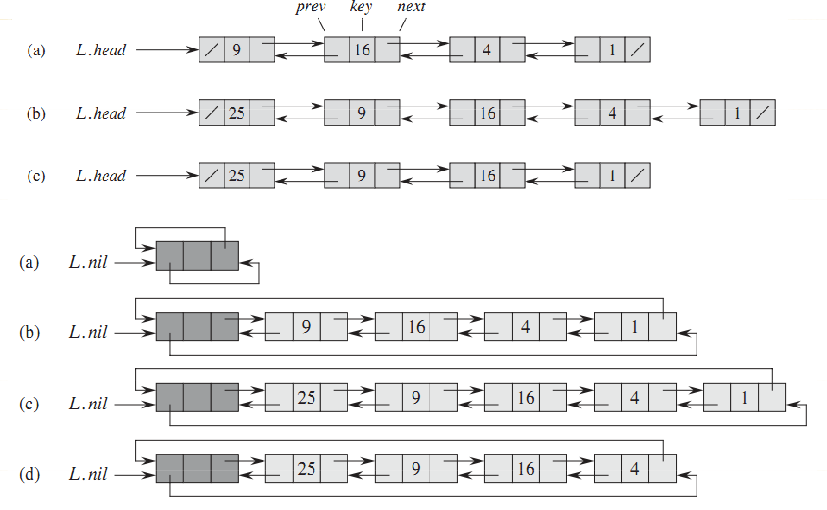
\includegraphics[scale=0.5]{../images/linkedlist.png}
\label{paging}
\end{center}
\end{figure}
\subsection{Trees}
We can use reference pointers and logical operations similar to that of linked lists to create rooted trees. The most elementary of these tree structures is a {\bf binary tree}. Each node of a binary tree has a possibly null ancestor and two possibly null children, left and right. This concept can be extended to create rooted trees with unbounded branching. These are known as $k-Ary$ trees, where $k$ may be fixed or totally unbounded. Figure \ref{kary} shows a rooted $k$-Ary tree. We will come back to trees once we have discussed algorithms in more detail.
\section{Algorithm}
 \begin{figure}
\caption{A k-ary tree structure.\cite{OSCONCEPTS}}
\begin{center}
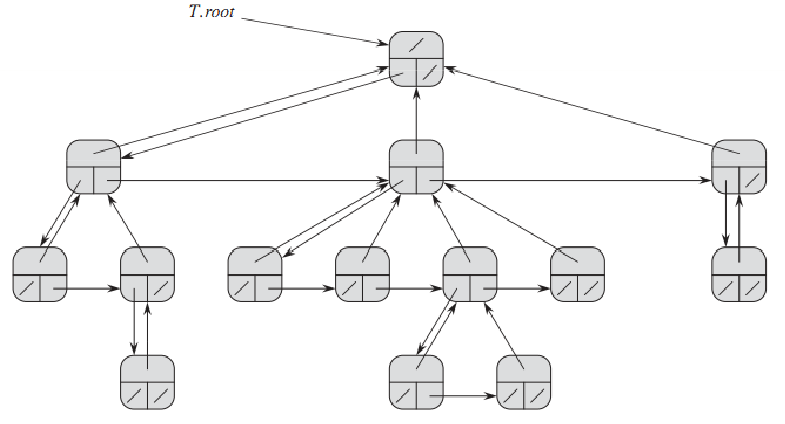
\includegraphics[scale=0.5]{../images/kary.png}
\label{kary}
\end{center}
\end{figure}

\section{Introduction to Algorithms}
An algorithm is any well defined computational procedure that takes some value or set of values as input and produces output. Practically, algorithms are sequences of computational steps that accomplishes this. More loosely, an algorithm is a tool for soliving some well-specified computation problem. A common computational problem that we will look at in detail is that of sorting a sequence of $n$ numbers $a_1,a_2...a_n$ producing $a'_1,a'_2...a'_n$ such that $a_1 <= a_2 <= ... <= a_n$. Each unique input and resulting output is known as an instance of the problem. 
\newline\newline
An algorithm is {\bf correct} if for every input instance, it halts with the correct output, thus solving the given computational problem. For this course, we are particularly interested in correct algorithms, however incorrect algorithms are useful if we can control their error rates. 
\newline\newline
Algorithms can be found accross multiple disciplines, from interent architectures that efficently route large volumes of data to graphics engines that render scenes in games. Understanding algorithms and their analysis is a fundamental skill that is expected of all programmers. Combining this general understanding with a suite of specific algorithms that are commonly applied in various guises is an extremely valuable addition to your skillset as a programmer. 
\newline\newline
Data-structures facilitate access and modification of dynamic sets, and therefore facilitate algorithm execution. None is fit for all purposes, so often the choice of algorithm is tightly coupled with the choice of data-structure used. 


<<< SOMETHING ON HARDNESS/SPACE VS TIME HERE >>>>

\subsection{Insertion Sort}
This is the first sorting implementation we we look at. Remember, the objective is to sort a sequence of $n$ numbers $a_1,a_2...a_n$ producing $a'_1,a'_2...a'_n$ such that $a_1 <= a_2 <= ... <= a_n$. We can refer to these numbers as keys in a data-structure, in this particular case we will choose an array of $n$ elements. Insertion sort is an aefficent algorithm for sorting a small number of elements, and is quite simple to understand. 
\newline\newline
Insertion sort works in a similar fashion to the way people normally sort a deck of cards by hand. In other words, we start with an empty left hand, with cards face down. Thereafter, we remove one card at a time from the table and insert it into the correct position of the left hand. Insertion sort will sort the input array {\bf in place} therefore re-arranging the numbers within the input array. There is a good insertion sort animation here \cite{INSANIM}. A fully worked example is shown in figure \ref{insertionlisting}
\begin{figure}
\caption{An example insertion sort.\cite{OSCONCEPTS}}
\begin{center}
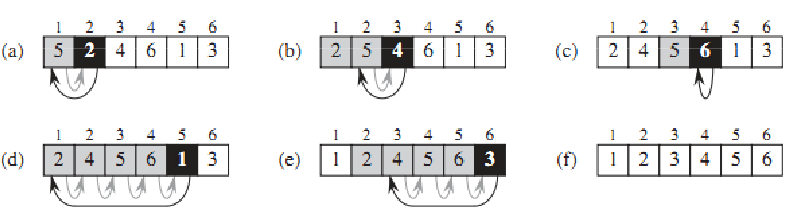
\includegraphics[scale=0.5]{../images/insertion.png}
\label{insertion}
\end{center}
\end{figure}
\begin{figure}
\caption{Insertion Sort}
\begin{center}
\begin{lstlisting}
INSERTION-SORT(A)
for j = 2 to A.length
  key = A[j]
  i = j-1
  while i > 0 and A[i] > key
    A[i+1]=A[1]
    i=i-1
  A[i+1]=key
\end{lstlisting}
\label{insertionlisting}
\end{center}
\end{figure}
We can formally examine the listing in \ref{insertionlisting} using a general framework. Firstly, we will define a {\bf loop invariant}. This is a statement of the conditions that should be true on an entry to a loop and are guaranteed to remain true on every further iteration of the loop. That is to say a loop invariant must be true at {\bf initialization}, at {\bf maintenence} and also at {\bf termination}.
\newline\newline
For insertion sort, the invariant is defined as $A[1...j-1]$ containing sorted elements, with the remaining elements unsorted. We can see this is true at initialization because we start off with $j=2$ therefore meaning $A[1...j-1]$ has only one element, and is thus implicitly sorted. At maintenence, every time we increment j we ensure that $A[1...j-1]$ will have more elements but that these elements will remain sorted relative to each other. Finally, we terminate at j == A.lenght, thus asserting that we have visited all elements. $A[1...j-1]$ is now equal to $A[1...n]$ and therefore the full array is sorted. 
\subsection{Analysis of Algorithms}
Approximating the resources that and algorithm consumes is important. For insertion sort, time taken to complete depends in some way on the input. Intuitively, we can see that sorting 1,000 numbers will take more iterations and therefore more processing time that sorting 3 numbers. Furthermore, insertion sort can take longer to sort two input sequences of the same size depending on how nearly sorted the are. We describe the time taken by an algoirthm to complete as a function of the size of its input $n$. The {\bf running time} of an algorithm on a particular input is therefore directly proportional to the number of steps executed by the algorithm. Assume that each operation takes $c$ time where $c$ is known as a {\bf constant factor}. The running time for the algorithm is the sum of running times for each statement. For insertion sort, we see the best case running time is a linear function captured as $an + b$. Conversely, if the input array is inverse-sorted then running time becomes $an62+bn+c$ which is a quadratic function.
\newline\newline
We are concerned with the {\bf asympptotic} efficency of algorithms, that is, how the running time of an algorithm increases with the size of the input, as the size of the input increases without bound. The algorithm that is asymptotically more efficent will usually be the best choice for all but very small inputs. Theta notation asymptotically bounds a function from above and below, however, we are usually concerned with only an asymptotic uppder bound. For this we use {\bf O-notation}. Using O-notation, we can often de4scribe the running time of an algorithm merely by inspecting the algorithms overall structure. For example, the doubly nested loop structure of insertion sort immediatedly yeields O(n2) upper bound with each execution of the loop executing in constant time. Theta notation for insertion sort has two figures, i.e. the theta(n2) worst case bound and the theta(n) best case bound. The latter, lower asymptotic bound can be expressed as omega(n) for insertion sort. s
\subsubsection{Worst Case Running Time}
The worst case running time is defined as the upper bound on running time for any input and provides us a guarantee that the algorithm will not take any longer. When considering running times of algorithms where we know nothing about our input set {\it a priori}, this is the quantification we focus on. Worst case occurs often enough for this to be a good rule of thumb. An example operation that is guaranteed to run in worst case time is searching through a list of keys for a value that is not in the list. 
\subsubsectionh{Best Case Running Time}
\subsubsection{Average Case Running Time}
When compared to worst case running time, the average case often roughly as bad as the worst case. For insertion sort, if the array is half unsorted then on average we still iterate over half of the sub-array. This is still a quadratic function. 
\subsubsection{Theta Notation}
\subsubsection{Big-O Notation} 

\subsection{Time Complexity}

O(1) - Constant Time - Hash-Table Array Lookup
O(logn) - Logarithmioc time - Finding an item in an array using binary search.
O(n) - Linear Time
O(n log n) or O(log n!) - Quasi Linear - Merge, Quick and Heap Sort
O(n2) - Quadratic - Insertion Sort
O(nc) - Polynomial -
O(cn) - Exponential - 
O(n!) - Factorial - Traveling Salesman by brute force search.

\subsection{Space Complexity}


\subsection{Designing Algorithms}
There are a huge number of ways to design algorithms, but we will talk about two general classes. The first class takes the {\bf incremental} approach, whereby we progress in increments through the steps required. The other class we will consider is the class of algorithms that take the {\bf divide and conquer} approach. These algorithms use the concept of a {\bf recursive structure} to solve the larger problem by solving the set of sub problems contained within the problem itself. At each level of recursion we {\bf divide} the problem into a number of smaller sub-problems, which are instances of the same problem. We conquer the sub-problems by solving them recursively, until the problem size is small enough to either solve incrementally efficently or solve trivially. Thereafter we {\bf combine} the solutions  to the sub-problems into the solution for the original problem. The second approach lends itself well to parallelism, although this is not the only motivating factor in choosing the approach. 
\newline\newline
Recursion is the process of repeating in a self similar way. In computer science and in practical terms, recursion is where a procedure or function calls itself, typically with modified parameters from the inital execution. This approach is used typically in dividing problems into sub-problems. The listing in figure \ref{faclisting} illustrates a recursive factorial function. 

\begin{figure}
\caption{Recursion}
\begin{center}
\begin{lstlisting}
private int factorial{int n} {
  if (n<=1) 
    return 1;
  else 
    return n * factorial(n-1);
}
\end{lstlisting}
\label{faclisting}
\end{center}
\end{figure}

\subsection{Merge Sort}
Insertion sort is an example of an incremental algorithm. Merge sort takes the divide and conquer approach. First we divide an n-element sequence into sub-sequences of $n/2$ elements each. Next, we sort the two sub-sequences recursively using merge-sort, which itself will cause sub-divides until the size of the sub-divided arrays is 1. The recursion {\bf bottoms out} in this case and we then merge all sorted sub-sequences by unwinding the recursion tree. The solution is the combined set of sorted sub-sets. 
\begin{figure}
\caption{Merge-Sort}
\begin{center}
\begin{lstlisting}
MERGE(A, p, q, r)
# A the array to sort
# p, q and r are indices into the array sucha that p<=q<r
# Assuming sub arrays A[p...q] and A[q+1..r] are sorted
# we merge them to form a single sorted sub-array. 
N1 = q - p + 1
N2 = r - q
let L[1..n1+1] and R[1..n2+1] be new arrays
for i = 1 to n1
  L[i]=A[p+1-1]
for j = 1 to n2
  R[j]=[A+q+j]
L[n1+1]=NIL
R[n2+1]NIL
i=1
j=1
for k = p to r
if L[i] <= R[j]
  A[k]=L[i]
  i=i+1
else
  j=j+1
\end{lstlisting}
\begin{lstlisting}
MERGE-SORT(A, p, r)
if p < r
  q = [(p+r)/2]
  MERGE-SORT(A,p,q)
  MERGE-SORT(A,q+1,r)
  MERGE(A,p,q,r)
\end{lstlisting}
\label{mslisting}
\end{center}
\end{figure}
\begin{figure}
\caption{Merge Sort\cite{OSCONCEPTS}}
\begin{center}
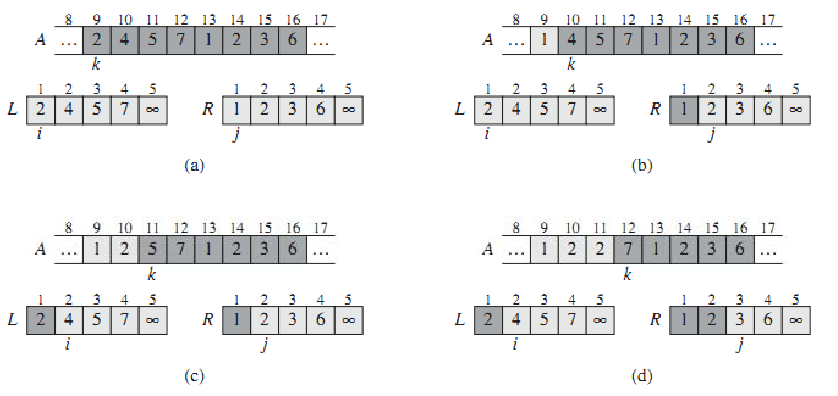
\includegraphics[scale=0.5]{../images/mergesort.png}
\label{mergesort}
\end{center}
\end{figure}
\end{figure}
\begin{figure}
\caption{The full recursion tree of a merge sort example\cite{OSCONCEPTS}}
\begin{center}
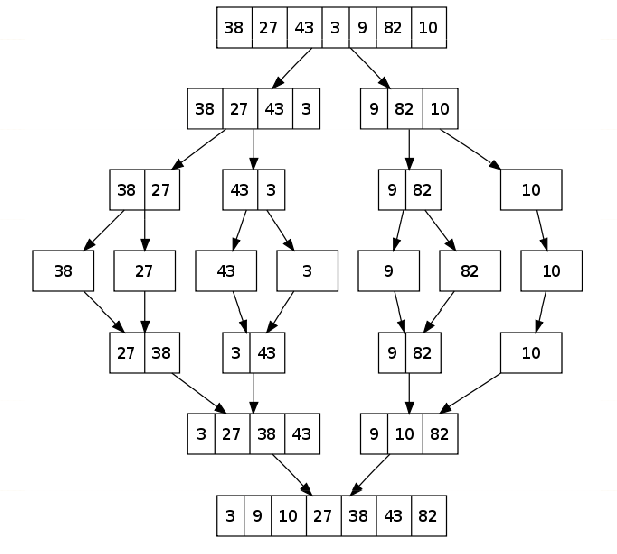
\includegraphics[scale=0.5]{../images/rmergesort.png}
\label{rmergesort}
\end{center}
\end{figure}
Figure \ref{mslisting} shows the code required to implement merge sort and figure \ref{mergesort} colors this detail with an example merge operation. Figure \ref{rmergesort} shows the full divide, conquer and merge recursion tree. 
\subsubsection{Loop Invariant}
The sub-array A[p..k-1] contains the k-p smallest elements of L[1..n1+1] and R[1..n2+1] in sorted order. L[i] and R[j] are the smalles elements of their arrays that have not been copied back to A. 
\subsubsection{Initialization}
Since k=p that makes A[p..k-1] empty. Thus the $k-p$, or 0, smalles elements of L and R are in L and R since i=j=1.
\subsubsection{Maintenance}
If L[i]<=R[j] then L[i] is the smalles element not copied back into A. A[p..k01] contains the k-p smalles elements after line 14 copies L[i] into A[k] leaving the sub-array A[p..k] which will conatin the k-p+1 smallest elements. Incrementing k reinitializes the loop invariant for the next iteration. For L[i]>R[j] lines 16 and 17 maintain the loop invariant.
\subsubsection{Termination}
At termination k=r+1. The subarray A[p..k-1] which is A[p..r] contains the k-p=r-p+1 smalles elements ofL[1..n1+1] and R[1..n2+1] in sorted order. Land R together contain N1+n2+2=r-p+3 elements. All but the two largest elements have been copied bac into A. These are the two senteniels (which is what exactly?)
\subsection{Analysis}
Theta(n) time for the merge procedure. Lines 1-3 and 8-11 take constant time whereas the for loops of lines 4 to 7 take O(n1+n2) time. When algorithms contain recursive calls to itself we describe running time by a recurrence equation. This describes the overall running time on a problem of size n in terms of the running time on smaller inputs. Solving these recurrences can help us put bounds around the performance of the algorithm. For merge-sort we have O(n log n) worst case and average time. Most implementations use a {\stable sort} which does not change the order of equal keys in meory. Mergsort uses O(n) space complexity. 
\newline\newline\subsection
Insertion sort runs in O(n) best case time and O(n2) worst and average time. This is reasonably efficent for mall data sets. Since it is an {\bf in-place} sort, the space complexity is O(1). Insertion sort is fully stable. Insertion sort is typically used to sort small arrays. 

\bibliography{../biblio/techfundamentals.bib}{}
\bibliographystyle{plain}
\begin{center}
{\small \copyright  David Lynch 2012. Do not reproduce without written permission.}
\end{center}
\end{document}
